\section{Numerisches Lösen von DGL}

\subsection{Das Euler Verfahren}
DGL 1. Ordnung mit Anfangswert:
\begin{equation*}
    \tikzmark{a}\dot{x} = f(\tikzmark{b}t,x), \hspace{1em} x(0)=x_0
\end{equation*}
\begin{center}
    \begin{tikzpicture}[overlay,remember picture]
        \node at (-4,0) (ta) {Steigung};
        \node[right] at (-2,0) (tb) {Entspricht Funktion $f$ der gesuchten Variable $x$};
        \draw[->] (ta) [in=-90]to (a);
        \draw[->] (tb) [in=-90,out=100]to (b);
    \end{tikzpicture}
\end{center}
Idee: Immer nur ein Schritt auf einmal.
\begin{center}
    \begin{tikzpicture}
        \draw (-1,0) -- (0,0) -- (0,-1);
        \draw[<->] (6,0) node[below] {$t$} -- (0,0) -- (0,3) node[left] {$x$};
        \draw[thick] (0,1) node[left] {$x_0$} -- ++ (3,0) -- ++ (0,1)
        node[midway, right] {$\Delta x$}   -- (0,1);
        \draw (3,-0.1) node[below] {$t_1$} -- (3,0.1);
        \draw (0.1,2)  -- (-0.1,2) node[left] {$x_1$};
        \node[below] at (1.5,0) {$\Delta t = h$};
        \node at ( 7,2) {$\dfrac{\Delta x}{h} = f(t,x_0)$};
    \end{tikzpicture}
\end{center}
Explizites Euler Verfahren:
\begin{equation*}
    \boxed{
        x_{n+1} = x_n + h\cdot f\left( t_n,x_n \right)
    }
\end{equation*}
Implizites Euler Verfahren:
\begin{equation*}
    \boxed{
        x_{n+1} = x_n + h\cdot f\left( t+h,x_{n+1} \right)
    }
\end{equation*}

\bsp{Beispiel:}
Gegeben ist die DGL
\begin{equation*}
    \dot{x} = x^2+2t\cdot x, \hspace{1em} x_0 = 2
\end{equation*}
Nicht linear und nicht separierbar $\Rightarrow$ numerisch lösen.

Expliziter Euler mit Schrittweite $h=1$:
\begin{eqnarr}
    \dot{x} &=&  f(t,x) \\
    &=&  x^2+2t\cdot x\\
    &\Rightarrow&\\
    x_{n+1} &=& x_n + h\cdot \left( x_n^2+2t_n\cdot x_n \right)\\
    x_{1} &=& x_0 + h\cdot \left( x_0^2+2t_0\cdot x_0 \right)\\
    &=& 2 + 1\cdot \left( 2^2+2\cdot 0 \cdot 2 \right)\\
    &=& 6\\
    x_2 &=&  x_1 + h\cdot \left( x_1^2+2t_1\cdot x_1 \right)\\
    &=& 6 + 1\cdot\left( 6^2+2\cdot 1\cdot 6 \right)\\
    &=& 54\\
    \text{usw.}&&\\
\end{eqnarr}

\subsection{Runge-Kutta Verfahren}
\subsubsection{Runge-Kutta 2}
(Mittelpunktsregel)
\begin{eqnarr}
    x_{n+\frac{1}{2}} &=&  x_n + \frac{h}{2}\cdot f\left( t_n,x_{n} \right)\\
    x_{n+1} &=& x_n + h\cdot f\left(t_n+\frac{h}{2},x_{n+\frac{1}{2}}\right)\\
\end{eqnarr}
\begin{center}
    \begin{tikzpicture}
    \begin{axis}[
        width = 10cm,
        height = 5cm,
        axis lines = middle,
        clip = false,
        xmin = 0,
        xmax = 6,
        ymin = 0,
        ymax = 6, 
        restrict y to domain=0:6,
        ticks=none,
        xlabel = $t$,
        ylabel = $x$,
    ]

    \addplot+[mark=none,samples=50,domain=0:6 ] {x^2/3}
    node[pos=0.9,below right] {$x=\dfrac{1}{3}t^2$};
    \addplot[mark=none,samples=5,domain=1.5:2.5 ] {4*x/3-4/3};
    \addplot[mark=none,samples=5,domain=0:6 ] {4*x/3};

    \draw (axis cs:2,0.1) -- ++(axis cs:0,-0.2) node[below] {$t_{n+\frac{1}{2}}$};
    \draw (axis cs:4,0.1) -- ++(axis cs:0,-0.2) node[below] {$t_n$};
    
\end{axis}
    \end{tikzpicture}
\end{center}

\subsubsection{Runge Kutta 4}
(Klassisches Runge Kutta)
\begin{eqnarr}
    x_{A} &=&  x_n + \frac{h}{2}\cdot f\left( t_n,x_{n} \right)\\
    x_{B} &=&  x_n + \frac{h}{2}\cdot f\left( t_n+\frac{h}{2},x_{A} \right)\\
    x_{C} &=&  x_n + h\cdot f\left( t_n+\frac{h}{2},x_{B} \right)\\
    x_{n+1} &=& x_n + \frac{h}{6}\cdot \left( 
        f\left( t_n,x_{n} \right) + 2\cdot \left( 
        f\left( t_n+\frac{h}{2},x_{A} \right) \right.\right. +\\
        && \left.\left.   f\left( t_n+\frac{h}{2},x_{B} \right)
        \right) +
            f\left( t_n+h,x_{C} \right)
    \right)
\end{eqnarr}

\bsp{Beispiel:}

$\dot{x} = -x+\cos(t)$
\begin{center}
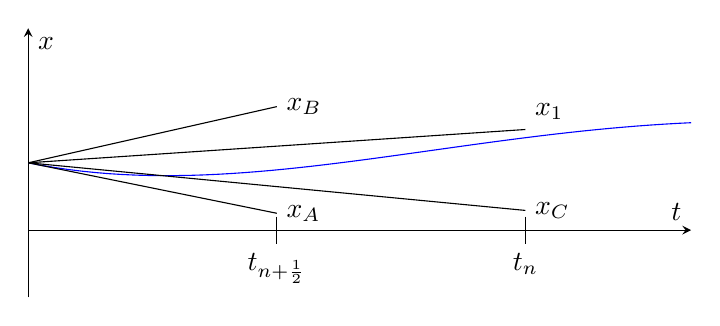
\begin{tikzpicture}
\begin{axis}[
        width = 10cm,
        height = 5cm,
        axis lines = middle,
        clip = false,
        xmin = 0,
        xmax = 2,
        ymin = -0.5,
        ymax = 1.5, 
        restrict y to domain=-4:7,
        ticks=none,
        xlabel = $t$,
        ylabel = $x$,
    ]

    \pgfmathdeclarefunction{ffunc}{2}{%
        \pgfmathparse{%
            -#2+sin(deg(#1))
        }%
    }
    \pgfmathdeclarefunction{xfunc}{1}{%
        \pgfmathparse{%
            exp(-#1) + sin(deg(#1))/2-cos(deg(#1))/2
        }%
    }

    \addplot+[mark=none,samples=50,domain=0:2 ] {xfunc(x)};
    %node[pos=0.5,below right] {$x=\sin(t)+2$};
    \addplot[mark=none,samples=5,domain=0:0.75] {ffunc(0,0.5)*x+0.5}
    node[right] (xa) {$x_A$};
    \addplot[mark=none,samples=5,domain=0:0.75] {ffunc(0.75,0.125)*x+0.5}
    node[right] (xb) {$x_B$};
    \addplot[mark=none,samples=5,domain=0:1.5] {ffunc(0.75,0.917479)*x+0.5}
    node[right] {$x_C$};
    \addplot[mark=none,samples=5,domain=0:1.5] {0.165*x+0.5}
    node[above right] {$x_1$};
    %\addplot[mark=none,samples=5,domain=0:4] {
        %4/6*(1.5*cos(deg(1.5*2)))
    %*x+2}
    %node[right] {$x_C$};

    \draw (axis cs:0.75,0.1) -- (axis cs:0.75,-0.1) node[below] {$t_{n+\frac{1}{2}}$};
    \draw (axis cs:1.5,0.1) -- (axis cs:1.5,-0.1) node[below] {$t_n$};
    
\end{axis}
\end{tikzpicture}
\end{center}

\subsection{Fehler}
Numerische Verfahren sind \underline{immer} Fehlerbehaftet
\begin{outline}
    \1 Rundungsfehler (z.B. Maschinenzahlen)
    \1 Diskretisierungsfehler
\end{outline}
\begin{center}
\begin{tikzpicture}
    \draw (-1,0) -- (0,0) -- (0,-1);
    \draw[<->] (6,0) node[below] {$t$} -- (0,0) -- (0,3) node[left] {$x$};
    \draw (0.1,1) -- ++ (-0.1,0) node[left] {$x_0$};
    \draw (2.5,0.1) -- ++ (0,-0.1) node[below] {$h$};
    \draw (5,0.1) -- ++ (0,-0.1) node[below] {$2h$};

    \draw[dotted] (0,1) 
                to[out=10,in=160] (2,0.5) 
                to[out=-20,in=180] (3,1)
                to[out=0,in=180] (4,0.4)
                to[out=0,in=200] (6,2) 
                node[right] {exakt}
                ;

    \draw (0,1) -- (2.5,2) -- (5,2.5) -- (6,3) node[right] {approx.};

    \draw[|-|] (2.5,2) -- ++ (0,-1.3) node[midway,left] {$e_1$};
    \draw[|-|] (5,2.5) -- ++ (0,-1.5) node[midway,left] {$e_2$};
\end{tikzpicture}
\end{center}

\textbf{Absoluter Fehler:}
\begin{equation*}
    e_{\text{abs}} = \left| x_{\text{num}} - x_{\text{exakt}} \right|
\end{equation*}
\textbf{Relativer Fehler:}
\begin{equation*}
    e_{\text{rel}} = \left| \frac{x_{\text{num}} - x_{\text{exakt}}}
                            {x_{\text{num}}}\right|
\end{equation*}
\textbf{Konvergenzordnung:}

Ein Verfahren besitzt Konvergenzordnung $n$, wenn der Fehler $e =
\mathcal{O}\left( h^n \right)$ ist.

\bsp{Euler Verfahren:}\\
Das Euler Verfahren besitzt Ordnung 1 $\Rightarrow$ Schrittweite halbieren
$\Leftrightarrow$ Fehler halbieren.

\subsection{Differentialgleichungssysteme}
Bis jetzt immer nur DGL 1.Ordnung. Was, wenn die DGL eine höhere Ordnung hat?

\bsp{Satz:}

Jede DGL n-ter Ordnung kann in ein System von n DGL 1.Ordnung umgeformt werden.

Vorgehen:
\begin{equation*}
\begin{array}{c}
    x^{(0)}\rightarrow x_0\\
    x^{(1)}\rightarrow x_1\\
    x^{(2)}\rightarrow x_2\\
    \vdots\\
    x^{(n)}\rightarrow x_n\\
\end{array}
\Rightarrow
\begin{array}{c}
    \dot{x}_0 = x_1\\
    \dot{x}_1 = x_2\\
    \dot{x}_2 = x_3\\
    \vdots\\
    \dot{x}_{n-1} = x_n\\
\end{array}
\Rightarrow
\begin{cases}
    \dot{\x} = A\x+\b, & \text{(Gleichungen linear)}\\
    \dot{\x} = f(\x),  & \text{(Gleichungen nicht-linear)}\\
\end{cases}
\end{equation*}

\bsp{Beispiel:}
\begin{equation*}
    \ddot{x}+8\dot{x}+25x=0
\end{equation*}
Schritt 1: Umbenennen
\begin{equation*}
    \begin{array}{c}
        x\rightarrow x_0\\
        \dot{x} \rightarrow x_1
    \end{array}
    \Rightarrow
    \begin{array}{l}
        \dot{x}_0 = \dot{x} = x_1\\
        \dot{x}_1 = \ddot{x}
    \end{array}
\end{equation*}
Schritt 2: In DGL einsetzen
\begin{eqnarr}
    \ddot{x}+8\dot{x}+25x&=& 0\\
    \dot{x_1}+8x_1+25x_0&=& 0\\
    \dot{x_1}&=& -8x_1-25x_0\\
\end{eqnarr}
Schritt 3: Als System von DGL schreiben:
\begin{equation*}
    \underbrace{
        \left[\begin{array}{c}
            \dot{x}_0\\
            \dot{x}_1
        \end{array}\right]
    }_{\dot{\x}}
    =
    \left[\begin{array}{c}
            x_1\\
            -8x_1-25x_0
    \end{array}\right]
    =
    \underbrace{
        \left[\begin{array}{cc}
                0 & 1\\
                -25 & -8
        \end{array}\right]
    }_{A}
    \underbrace{
        \left[\begin{array}{c}
                x_0\\
                x_1
        \end{array}\right]
    }_{\x}
\end{equation*}

\subsection{Matlab ode}
Das Lösen von DGL in Matlab geschieht numerisch, zum Beispiel mithilfe obiger 
Verfahren.

Eine mögliche Implementation des expliziten Euler-Verfahrens ist sehr
einfach:
\lstinputlisting{codes/explicitEuler.m}
